\section{Aplicación del método estático}
Inicialmente se considera los siguientes datos adjuntos en la siguiente imagen:

\begin{figure}[h!]
    \centering
    \begin{subfigure}[b]{0.54\linewidth}
    \centering
    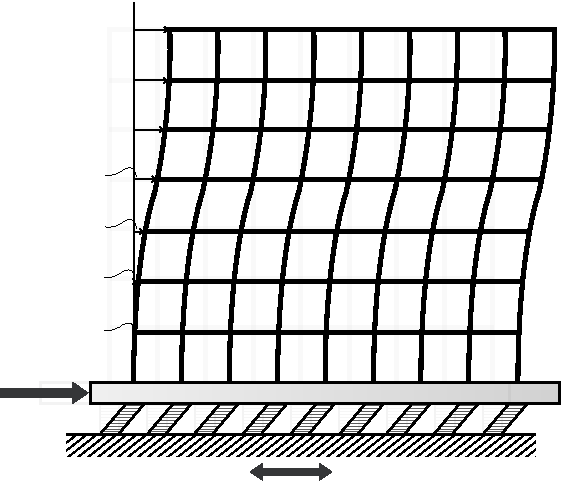
\includegraphics[width = \linewidth]{img/1-CAP/EDIF_1.pdf}
    \begin{tikzpicture}[remember picture, overlay]
        \node[align=center] at (-3.5,2.25) {$V_b$};
        \node[align=center] at (1.3,0.65) {$\ddot{u}_g(t)$};
        \node[align=center] at (-2,7.65) {\footnotesize$d_7$};
        \node[align=center] at (-2,6.9) {\footnotesize$d_6$};
        \node[align=center] at (-2,6.15) {\footnotesize$d_5$};
        \node[align=center] at (-2.95,5.25) {\footnotesize$d_4$};
        \node[align=center] at (-2.95,4.5) {\footnotesize$d_3$};
        \node[align=center] at (-2.95,3.7) {\footnotesize$d_2$};
        \node[align=center] at (-2.95,2.95) {\footnotesize$d_1$};
    \end{tikzpicture}
        \caption{}
        \label{i1_1.1}
    \end{subfigure}
    \hfill
    \begin{subfigure}[b]{0.32\linewidth}
        \centering
        
\includegraphics[width = \linewidth]{img/1-CAP/EDIF_2.pdf}
        \begin{tikzpicture}[remember picture, overlay]
            \node[align=center] at (0.1,4.8) {
            \begin{tblr}{
                colspec = {X[l, wd=4.5cm]},
                row{1,2,3,4,5,6,7} = {font = \small}
            }
                {\bfseries Amortiguamiento: \\ $\xi = 15\%$} \\
                
                {\bfseries Periodo de base fija: \\ $T_s = 1.2878 \; seg$} \\
                
                $- \circ -$ \\

                {\bfseries Masa superestructura: \\ $M_s = 2699.28 \; \frac{tonf-s^2}{m}$} \\

                {\bfseries Masa subestructura: \\ $M_b = 393.48 \; \frac{tonf-s^2}{m}$} \\

                {\bfseries Factores sísmicos:}
            \end{tblr}
            };
            \node[align=center] at (-1.67,1.3) {$0.45$};
            \node[align=center] at (-0.5,1.3) {$1.00$};
            \node[align=center] at (0.7,1.3) {$C_{(T)}$};
            \node[align=center] at (1.85,1.3) {$1.00$};
        \end{tikzpicture}
        \caption{}
        \label{i1_1.2}
    \end{subfigure}
    \caption[Datos del edificio analizado]{Datos del edificio analizado:
    \subref{i1_1.1} Vista en elevación en dirección $\vec{y}$;
    \subref{i1_1.2} Datos preliminares
    }
    \label{i1_1}
\end{figure}

\subsection{Desplazamientos máximos en la estructura}
Se emplearán los siguientes datos:
\begin{DATOS}{Datos}
    \begin{itemize}
        \item Se asume un periodo objetivo igual a tres veces el periodo de base fija: $T_b = 3T_s = 3 \cdot 3.12878 = 3.8634 \; seg$
        \item La masa total del sistema estructural es: $M_t = M_s + M_b = 3092.76 \; \frac{tonf-s^2}{m}$
        \item La rigidez de la superestructura es: $K_s = \left( \dfrac{2\pi}{3.863} \right)^2 \cdot (3092.75) = 8180.22 \; \frac{tonf}{m}$
    \end{itemize}
\end{DATOS}

\subsubsection{Desplazamiento máximo traslacional del nivel de aislamiento}

De acuerdo al apartado 20.1 de la Norma E.031\supercite{E031.1}, el desplazamiento mínimo que debe soportar la estructura tiene la siguiente expresión:
\begin{equation}
    D_M = \dfrac{S_{aM} \cdot {T_b}^2}{4 \pi^2 \cdot B_M}
    \label{eq1_1}
\end{equation}
La expresión anterior puede reescribirse de la siguiente forma:
\begin{equation}
    S_d = \dfrac{S_{aM}}{\omega^2} \; \ldots \; \left(\omega = \frac{2\pi}{T_b}\right) \label{eq1_2}   
\end{equation}
La expresión corregida por el factor de amortiguamiento es:
\begin{equation}
    D_M = \dfrac{S_d}{B_M} \label{eq1_3}
\end{equation}
Donde: 
\begin{itemize}
    \item{\makebox[0.8cm][l]{$D_M$}}: desplazamiento máximo traslacional
    \item{\makebox[0.8cm][l]{$S_{aM}$}}: ordenada máxima del espectro de pseudo-aceleraciones
    \item{\makebox[0.8cm][l]{$T_b$}}: periodo objetivo de la estructura aislada
    \item{\makebox[0.8cm][l]{$\omega$}}: velocidad angular de la estructura aislada
    \item{\makebox[0.8cm][l]{$B_M$}}: factor de corrección por amortiguamiento
\end{itemize}

Los espectros de pseudo-aceleraciones y pseudo-desplazamientos de la norma según los factores sísmicos se muestran a continuación:
\begin{figure}[h!]
    \centering
    \begin{subfigure}[b]{0.48\linewidth}
        \centering
        \begin{tikzpicture}
        \begin{axis}[
            xtick={0, 0.5, 1, 1.5, 2, 2.5, 3, 3.5, 4, 4.5, 5},
            ytick={0, 0.2, 0.4, 0.6, 0.8, 1, 1.2, 1.4, 1.6, 1.8},
            width=7.8cm, height=6.5cm,
            xlabel={$T \; (seg)$},
            ylabel={$S_a \; (g)$},
            label style={font=\footnotesize},
            tick label style={font=\tiny},
            x label style={at={(axis description cs: 0.5,0)},anchor=north},
            y label style={at={(axis description cs:0,.5)},anchor=north},
            %rotate=90,
            grid style={line width=.1pt, draw=gray!10},
            major grid style={line width=.2pt,draw=gray!50},
            grid = both,
            minor tick num=1,
            xmin = 0.0,
            xmax = 5,
            ymin = 0,
            ymax = 1.8,
            clip=false,]
            %COMPONENTE IMPULSIVA
        \addplot [black,mark=none, line width = 1.25pt] table[col sep=comma] {ESPEC_NORMA/ESPECTRO_E031.csv};
        \draw[line width=0.3mm, dashed, black] (axis cs: 0.08,\pgfkeysvalueof{/pgfplots/ymin}) -- (axis cs: 0.08,\pgfkeysvalueof{/pgfplots/ymax})node[anchor=west,rotate=90]{\tiny $0.2T_P = 0.08 \; s$};
        \draw[line width=0.3mm, dashed, black] (axis cs: 0.4,\pgfkeysvalueof{/pgfplots/ymin}) -- (axis cs: 0.4,\pgfkeysvalueof{/pgfplots/ymax})node[anchor=west,rotate=90]{\tiny $T_P = 0.4 \; s$};
        \draw[line width=0.3mm, dashed, black] (axis cs: 2.5,\pgfkeysvalueof{/pgfplots/ymin}) -- (axis cs: 2.5,\pgfkeysvalueof{/pgfplots/ymax})node[anchor=west,rotate=90]{\tiny $T_L = 2.5 \; s$};
        \draw[pline,blue,line width=0.75pt] plot coordinates {(386.34,0) (386.34,11.31)};
        \draw[pline,blue,line width=0.75pt] plot coordinates {(0,11.31) (386.34,11.31)};
        \node[text=blue] at (axis cs: 3.8634,0.2) {\fontsize{9}{9}\selectfont$\left(T_b, S_{aM}\right)$};
        \end{axis}
      \end{tikzpicture}
      \caption{}
      \label{i1_2.1}
  \end{subfigure}
  \hfill
  \begin{subfigure}[b]{0.48\linewidth}
    \centering
    \begin{tikzpicture}
        \begin{axis}[
            xtick={0, 0.5, 1, 1.5, 2, 2.5, 3, 3.5, 4, 4.5, 5},
            ytick={0, 50, 100, 150, 200, 250, 300, 350, 400, 450},
            width=7.8cm, height=6.5cm,
            xlabel={$T \; (seg)$},
            ylabel={$S_d \; (g)$},
            label style={font=\footnotesize},
            tick label style={font=\tiny},
            x label style={at={(axis description cs: 0.5,0)},anchor=north},
            y label style={at={(axis description cs:0,.5)},anchor=north},
            %rotate=90,
            grid style={line width=.1pt, draw=gray!10},
            major grid style={line width=.2pt,draw=gray!50},
            grid = both,
            minor tick num=1,
            xmin = 0.0,
            xmax = 5,
            ymin = 0,
            ymax = 450,
            clip=false,]
            %COMPONENTE IMPULSIVA
        \draw[pline,blue,line width=0.75pt] plot coordinates {(0,427.4487) (386.34,427.4487)};
        \draw[pline,blue,line width=0.75pt] plot coordinates {(386.34,0) (386.34,427.4487)};
        \addplot [black,mark=none, line width = 1.25pt] table[col sep=comma] {ESPEC_NORMA/Sd_ESPECTRO.csv};
        \node[text=blue] at (axis cs: 4.4,405) {\fontsize{9}{9}\selectfont$\left(T_b, S_d\right)$};
        \end{axis};
        \node[anchor=north] at (0.35,5.5) {\scriptsize$\times 10^{-4}$};
      \end{tikzpicture}
      \caption{}
      \label{i1_2.2}
  \end{subfigure}
  \begin{tikzpicture}[remember picture, overlay]
      \draw[black!55,->, bend left=30] (-8.5,7) to node[above] {$\div \omega^2$} (-7,7);
  \end{tikzpicture}
  \caption[Espectros de la norma según los parámetros sísmicos de la estructura]{Espectros de la norma según los parámetros sísmicos de la estructura:
  \subref{i1_2.1} Pseudo-aceleración;
  \subref{i1_2.2} Pseudo-desplazamiento}
  \label{i1_2}
\end{figure}

Primero se determina la pseudo-aceleración empleando la ecuación 5 de la Norma E.031\supercite{E031.2}.

\begin{itemize}
    \item Pseudoaceleración: $S_{a_{(T)}} = 1.50 \cdot Z \cdot U \cdot C_{(T)} \cdot S$
        \begin{itemize}
            \item [$\circ$] El valor de C es una función que depende del periodo y de las condiciones $T_P$ y $T_L$. Entonces, de acuerdo a la expresión $T = 3.86 > T_L = 2.50 \; seg$
            \begin{align*}
                C &= 2.50 \cdot \left( \dfrac{T_P \cdot T_L}{T^2} \right) = 2.50 \cdot \left( \dfrac{0.40 \cdot 2.50}{3.8634} \right) \\
                C &= 0.1675
            \end{align*}
            \item [$\circ$] $S_{a_{(T)}} = 1.50 \cdot 0.45 \cdot 1.00 \cdot 0.1675 \cdot 1.00 \cdot g = 0.113g = 110.911 \; cm/s^2$
        \end{itemize}
    \item Velocidad angular: $\omega = \frac{2\pi}{T_b} = \frac{2\pi}{3.863} = 1.626 \; rad/s \longrightarrow \omega^2 = 2.645$ 
    \end{itemize}

    Luego, el pseudo-desplazamiento se puede determinar empleando la ecuación \ref{eq1_2}:
    
    \begin{itemize}
    \item $S_d = \dfrac{Sa}{\omega^2} = \dfrac{110.911}{2.645} = 41.933 \; cm$
    \item Se aplica el factor de corrección por amortiguamiento $(B_M)$ según la tabla N\textdegree5 de la Norma E.031:
    
    \begin{minipage}[c]{0.45\linewidth}
    {\noindent Con amortiguamiento de $\beta_M = 15\%$:}
        \begin{align*}
            B_M &= \dfrac{B_{(20\%)} - B_{(10\%)}}{20\% - 10\%} \cdot (5\%) + B_{(10\%)} \\
            B_M &= \dfrac{1.50 - 1.20}{10\%}\cdot 5\% + 1.20 \\
            B_M &= \dfrac{0.30}{2} + 1.20 \\[3pt]
            B_M &= 0.15 + 1.20 \\[6pt]
            B_M &= 1.35
        \end{align*}
    \end{minipage}
    \hfill
    \begin{minipage}[c]{0.52\linewidth}
        \begin{longtblr}[
            caption = {Factor de amortiguamiento según la Norma E.031},
            label = {t1_1},
            note{*} = {\scriptsize Tomado de la tabla N\textdegree de la Norma E.031\supercite{E031.1}}
        ]{
            colspec = {X[c,m] X[c,m]},
            row{1} = {font = \bfseries\footnotesize,m},
            row{2,3,4,5,6,7,8} = {font = \footnotesize,m},
            hline{1,8} = {1pt},
            hline{2} = {0.25pt},
            row{3,5,7} = {gray!8},
        }
            {Amortiguamiento \\ $\bm{\beta_M}$} & {Factor \\ $\bm{B_M}$} \\

            $\leq 2\%$ & $0.80$ \\

            $5\%$ & $1.00$ \\

            $10\%$ & $1.20$ \\

            $20\%$ & $1.50$ \\

            $30\%$ & $1.70$ \\

            $\geq 40\%$ & $1.90$
        \end{longtblr}
    \end{minipage}\\ 

    {\noindent Entonces, la expresión corregida del desplazamiento traslacional es:}
    \begin{align*}
        D_M &= \dfrac{S_d}{B_M} = \dfrac{41.933}{1.35} \\[3pt]
        D_M &= 31.061 \; cm
    \end{align*}

    {\noindent Finalmente, el desplazamiento final corregido de acuerdo a la ecuación 16 de la Norma E.031\supercite{E031.3}}:
    \begin{align}
        D_M' &= \dfrac{D_M}{\sqrt{1 + \left(\dfrac{T_s}{T_b}\right)^2}} \; \ldots \; \epsilon = \left(\dfrac{T_s}{T_b}\right)^2 \nonumber \\[6pt]
        D_M' &= \dfrac{D_M}{\sqrt{1 + \epsilon}} \; \ldots \; ( \epsilon = 1/9) \label{eq1_4}
    \end{align}
    {\noindent Así, el desarrollo de la expresión tiene el siguiente resultado:}
    \begin{align*}
        D_M' &= \frac{D_M}{\sqrt{1 + \epsilon}} = \frac{31.061}{\sqrt{1 + 1/9}} \\[3pt] 
        D_M' &= 29.467 \; cm
    \end{align*}
    \end{itemize}
    
\subsubsection{Desplazamiento total en la base del aislamiento}
De acuerdo al inciso a) del apartado 20.3 de la Norma E.031\supercite{E031.4} el desplazamiento total debe incluir el desplazamiento adicional debido a la torsión. La figura \ref{i1_3} muestra la superposión de efectos que se considera en el desplazamiento total.
\newpage
\begin{figure}[h!]
    \centering
    \begin{subfigure}[b]{0.30\linewidth}
        \centering
        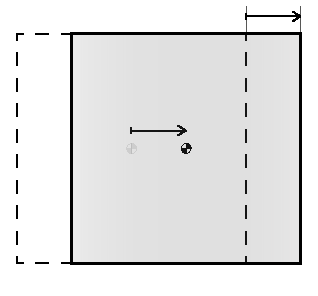
\includegraphics[width = \linewidth]{img/1-CAP/DM_1.pdf}
        \begin{tikzpicture}[remember picture, overlay]
            \node[align=center] at (0,3.2) {\footnotesize$D_M$};
            \node[align=center] at (1.9,5.2) {\footnotesize$D_M$};
            \node[align=center] at (0.5,2.4) {\footnotesize\bfseries C.G.};
        \end{tikzpicture}
        \caption{}
        \label{i1_3.1}
    \end{subfigure}
    \hfill
    \begin{subfigure}[b]{0.30\linewidth}
        \centering
        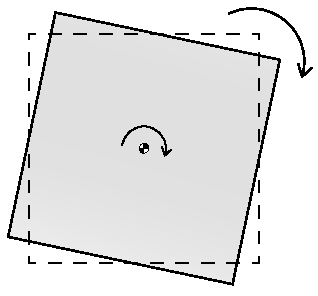
\includegraphics[width = \linewidth]{img/1-CAP/DM_2.pdf}
        \begin{tikzpicture}[remember picture, overlay]
            \node[align=center] at (0.4,2.85) {\footnotesize$\Delta\theta$};
            \node[align=center] at (2.55,4.1) {\footnotesize$\Delta\theta$};
            \node[align=center] at (-0.15,2.3) {\footnotesize\bfseries C.G.};
        \end{tikzpicture}
        \caption{}
        \label{i1_3.2}
    \end{subfigure}
    \hfill
    \begin{subfigure}[b]{0.30\linewidth}
        \centering
        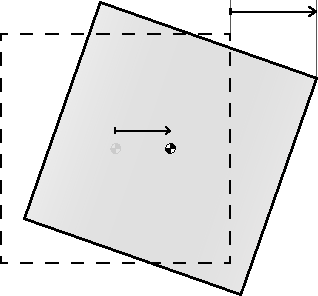
\includegraphics[width = \linewidth]{img/1-CAP/DM_3.pdf}
        \begin{tikzpicture}[remember picture, overlay]
            \node[align=center] at (-0.22,3.25) {\footnotesize$D_M$};
            \node[align=center] at (1.7,5.1) {\footnotesize$D_{TM}$};
            \node[align=center] at (0.2,2.4) {\footnotesize\bfseries C.G.};
        \end{tikzpicture}
        \caption{}
        \label{i1_3.3}
    \end{subfigure}
    \begin{tikzpicture}[remember picture, overlay]
        \node[align=center] at (-10.7,3.5) {\Large$\bm{+}$};
        \node[align=center] at (-5.7,3.5) {\Large$\bm{=}$};
    \end{tikzpicture}
    \caption[Desplazamiento total en función de los la superposición de movimientos]{Desplazamiento total en función de los la superposición de movimientos:
    \subref{i1_3.1} Traslacional;
    \subref{i1_3.2} Rotacional;
    \subref{i1_3.3} Desplazamiento total
    }
    \label{i1_3}
\end{figure}

Así, la expresión que permite determinar este valor es:
\begin{equation}
    D_{TM} = D_M \cdot \left[ 1 + \left( \dfrac{y}{{P_T}^2} \right) \cdot \left( \dfrac{12e}{b^2 + d^2} \right) \right] \label{eq1_5}
\end{equation}
Donde:
\begin{itemize}
    \item{\makebox[0.9cm][l]{$D_{TM}$}}: desplazamiento total del nivel de desplazamiento
    \item{\makebox[0.9cm][l]{$D_M$}}: desplazamiento máximo traslacional $(D_M = 29.467 \; cm)$
    \item{\makebox[0.9cm][l]{$y$}}: mitad de la distancia perpendicular de la dirección del análisis sísmico
    \item{\makebox[0.9cm][l]{$P_T$}}: razón entre el periodo traslacional y rotacional $\left( P_T = \frac{T_1}{T_3} = 1.08 \right) $
    \item{\makebox[0.9cm][l]{$e$}}: excentricidad entre el centro de masas y el centro de rigidez $(e = 5\% d)$
    \item{\makebox[0.9cm][l]{$b$}}: dimensión menor $(b = 56 \; m)$
    \item{\makebox[0.9cm][l]{$d$}}: dimensión mayor $(d = 63 \; m)$
\end{itemize}
Resolviendo:
\begin{align*}
    D_{TM} &= D_M \cdot \left[ 1 + \left( \dfrac{y}{{P_T}^2} \right) \cdot \left( \dfrac{12e}{b^2 + d^2} \right) \right] = 29.47 \cdot \left[ 1 + \left( \dfrac{63/2}{{1.08}^2} \right) \cdot \left( \dfrac{12 \cdot (5\% \cdot 63)}{56^2 + 63^2} \right) \right] \\
    D_{TM} &= 29.47 \cdot (1 + 0.14) \\
    D_{TM} &= 33.69 \; cm
\end{align*}

\subsection{Fuerza cortante máxima de la estructura}

\subsubsection{Fuerza cortante en la base de aislamiento}
La fuerza se determina según la ecuación 10 del apartado 21.1 de la Norma E.031\supercite{E031.5}.
\begin{equation}
    V_b = K_M \cdot D_M \label{eq1_6}
\end{equation}
Donde:
\begin{itemize}
    \item{\makebox[0.7cm][l]{$V_b$}}: fuerza cortante en la interfaz de aislamiento
    \item{\makebox[0.7cm][l]{$K_M$}}: rigidez efectiva de la interfaz de aislamiento $\left( K_M = K_s = 8180.24 \; \frac{tonf}{m} \right)$
    \item{\makebox[0.7cm][l]{$D_M$}}: desplazamiento máximo traslacional corregido $(D_M' = 29.467 \; cm)$
\end{itemize}
Resolviendo:
\begin{align*}
    V_b &= K_M \cdot D_M = 8180.24 \cdot 0.29467 \\
    V_b &= 2410.50 \; tonf
\end{align*}

\subsubsection{Fuerza cortante en la superestructura}
La fuerza se determina según la ecuación 12 del apartado 21.2b de la Norma E.031\supercite{E031.6}.
\begin{equation}
    V_{st} = V_b \cdot \left( \dfrac{P_s}{P}\right)^ {(1 - 2.5 \beta_M)} \label{eq1_7}
\end{equation}
Donde:
\begin{itemize}
    \item{\makebox[0.7cm][l]{$V_{st}$}}: fuerza cortante en la superestructura
    \item{\makebox[0.7cm][l]{$V_b$}}: fuerza cortante en la interfaz de aislamiento $(V_b = 2410.50 \; tonf)$
    \item{\makebox[0.7cm][l]{$P_s$}}: peso de la superestructura sin incluir el nivel de aislamiento $(P_s = 2699.28g)$
    \item{\makebox[0.7cm][l]{$P$}}: peso total incluyendo el nivel de aislamiento $(P = 3092.75g)$
\end{itemize}
Resolviendo:
\begin{align*}
    V_{st} &= V_b \cdot \left( \dfrac{P_s}{P}\right)^ {(1 - 2.5 \beta_M)} \\ 
    V_{st} &= 2410.50 \cdot \left( \dfrac{2699.28\cancel{g}}{3092.75\cancel{g}}\right)^ {(1 - 2.5 \cdot 0.15)} \\
    V_{st} &= 2213.96 \; tonf 
\end{align*}

